% !TEX root = ./main.tex

\section{Testbed: Many-Antenna Base Stations and Mobile Terminals}\label{sec:testbed}

Much the proposed research activities will leverage ArgosNet, a reconfigurable network research testbed with many-antenna MU-MIMO base stations recently funded by an NSF CRI grant.  
ArgosNet includes a configurable number of many-antenna base stations, ArgosBS, battery-powered mobile terminals based on ArgosMobile, and a server cluster connected to the base stations with high-throughout, precisely synchronized backhaul.  Currently ArgosNet supports real-time communication 2.4/5 GHz. Base stations will be precisely synchronized via the backhaul and cooperate to fully support network functions such as handoff and localization. 


\subsection{Argos: Reconfigurable and Scalable Base Station Architecture}\label{sec:argosv2}

\begin{figure*}[t]
%\vspace{-12mm}
\centering
\begin{minipage}[c]{0.62\textwidth}
\centering
 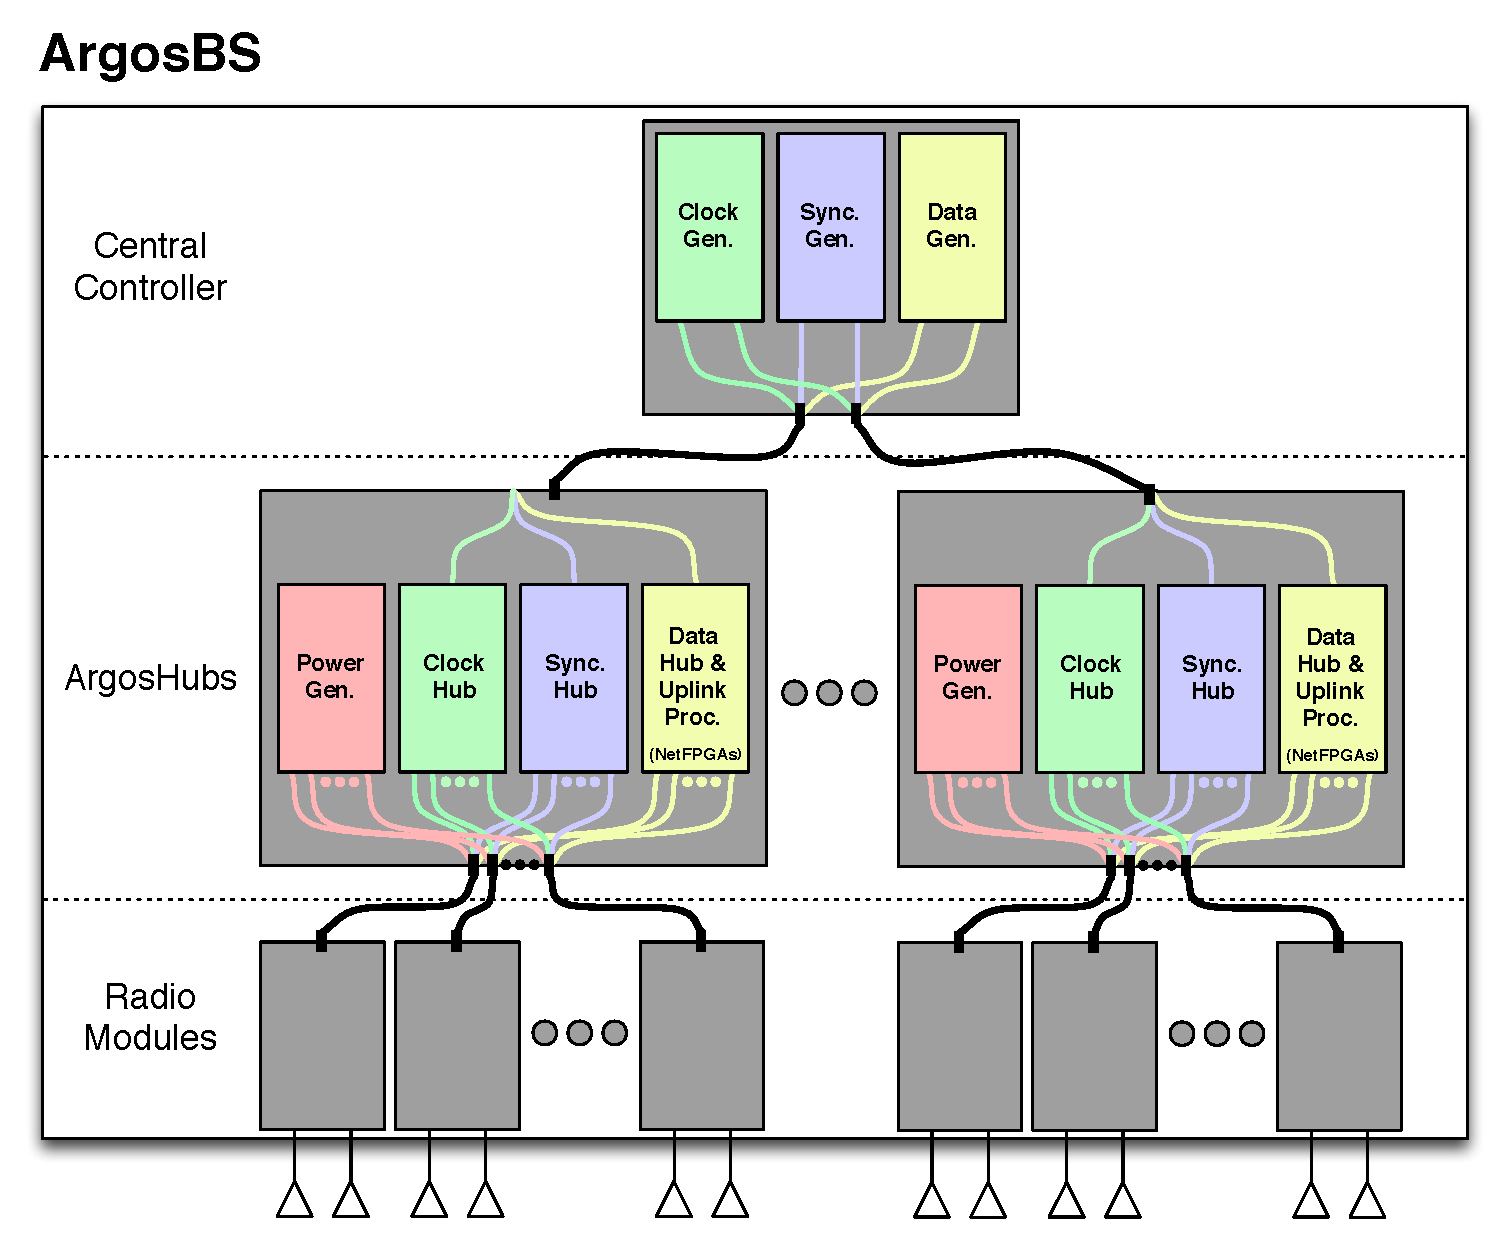
\includegraphics[width=\textwidth]{argosbs}
\end{minipage}
\hspace{2mm}
  \begin{minipage}[c]{0.34\textwidth}
  \centering
 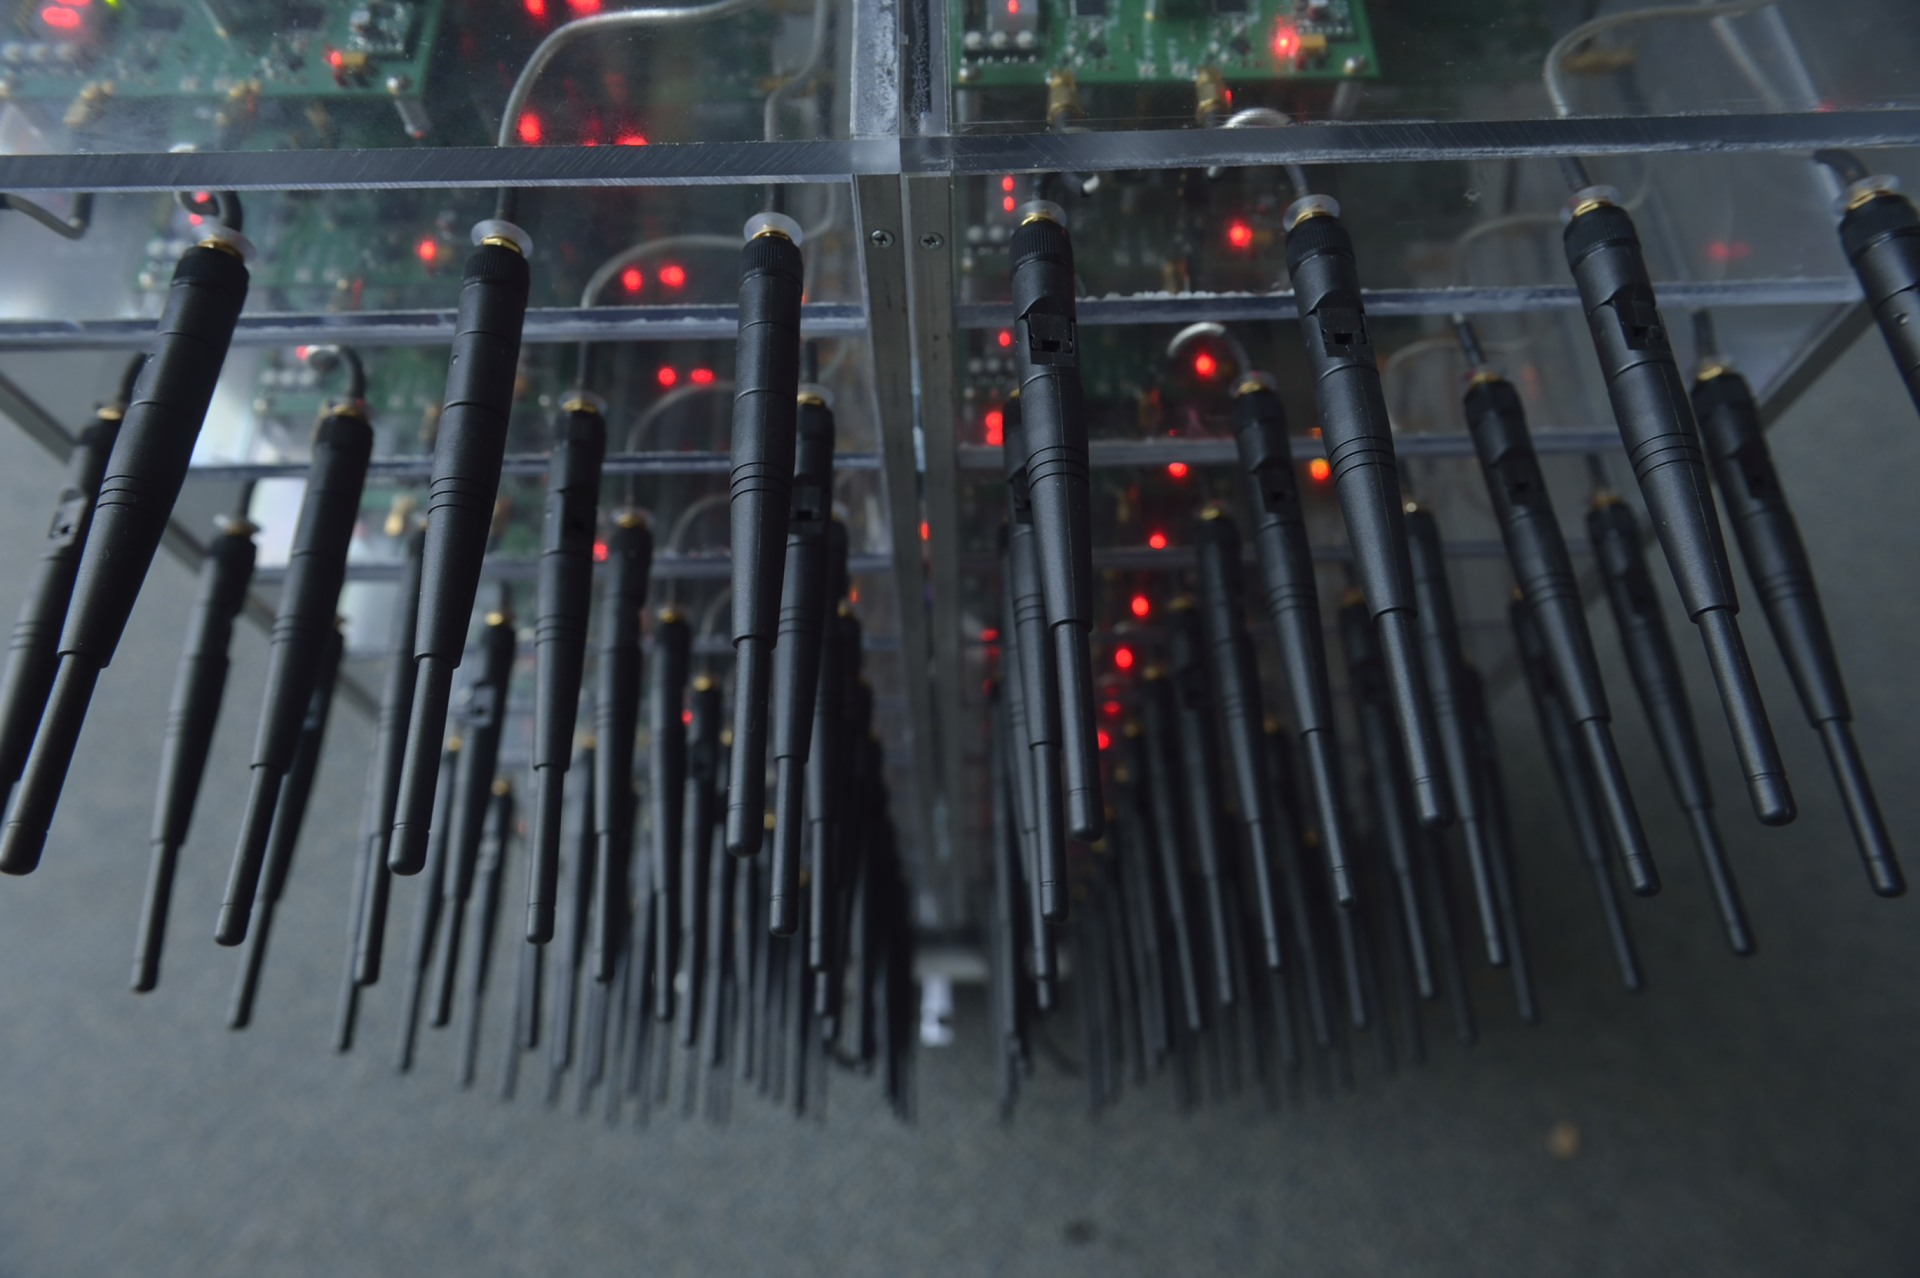
\includegraphics[width=\textwidth]{ArgosV2-Front-full}
 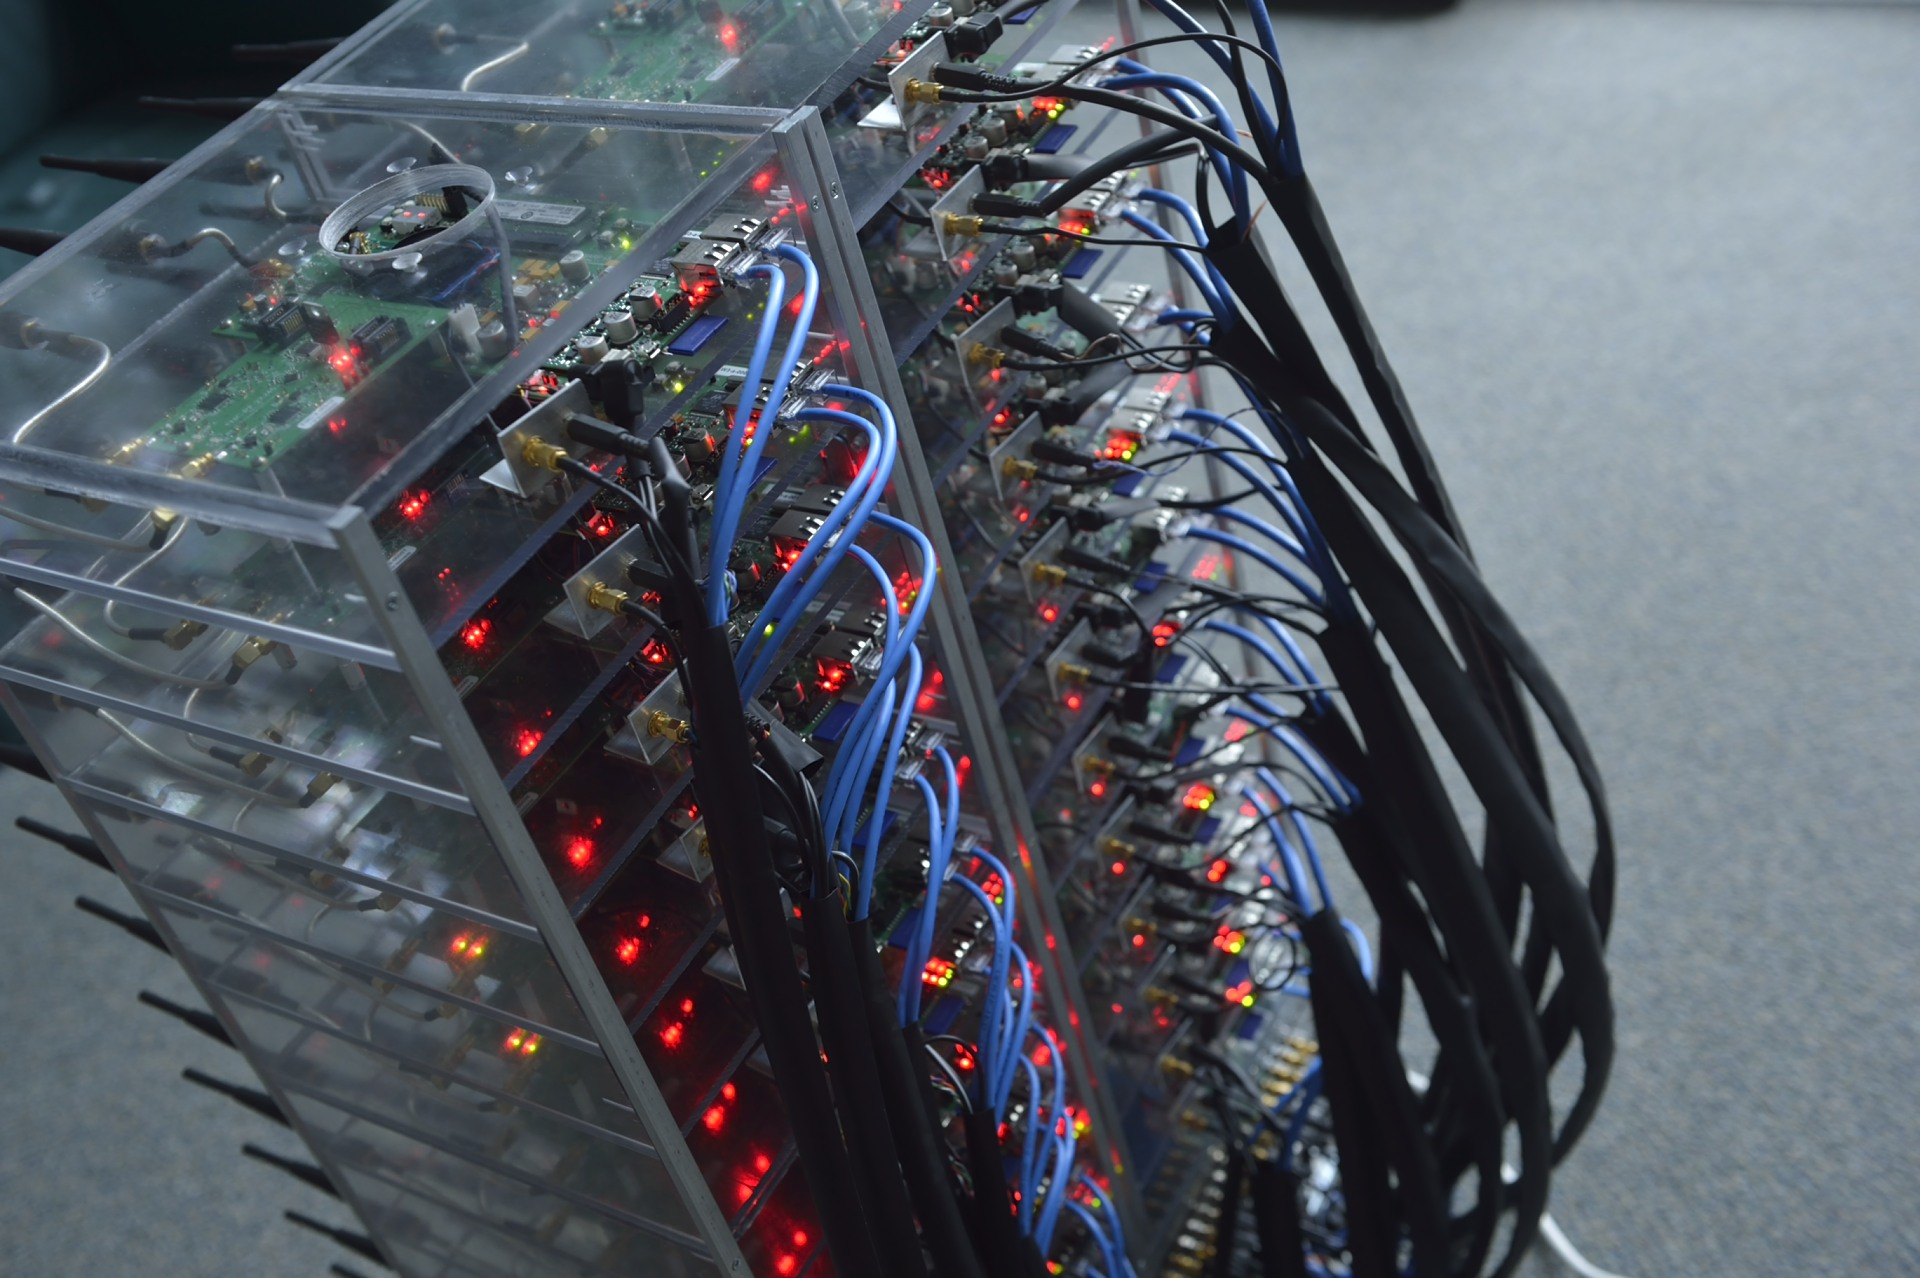
\includegraphics[width=\textwidth]{ArgosV2-Back-full}
 \end{minipage}
		\vspace{-2mm}
\caption{(left): \emph{The architecture of ArgosBS consists of a central controller, one or more ArgosHubs, and up to 100s of radio modules. 
			All links between blocks include a 10 GbE data link, a coaxial clock cable, and a twisted pair for timing synchronization. 
			ArgosHubs additionally supply power to their modules.} (right): \emph{Front and back views of ArgosV2 which features a refined modular mechanical design compared to ArgosV1 reported in~\cite{shepard2012mobicom}.} }
		\vspace{-2mm}
\label{fig:ArgosV2}
\end{figure*}

PI Zhong's group pioneered the design and prototyping of many-antenna base stations, producing two generations of the Argos base station architecture.
The first generation, presented in~\cite{shepard2012mobicom}, employed WARPv1 and supported 64 antennas serving 15 clients via MU-MIMO.  
It provided the first publicly reported experimental results of massive MIMO~\cite{shepard2012mobicom}.
 
The Argos architecture, depicted in Figure~\ref{fig:ArgosV2} (left),  is critical for realizing practical real-world massive-MIMO systems. 
It leverages a fat tree structure to optimize scalability, flexibility, and reliability, allowing massive-MIMO systems to scale to 1000s of antennas in the real world by taking in to account practical constraints. 
At the center of the architecture is the \emph{Central Controller} which is responsible for all layer 2 (MAC), as well as higher-level layer 1 operations, including scheduling, coding, modulation, and portions of MU-MIMO processing.
The central controller is connected to one or more \emph{ArgosHubs}, which distribute user data, maintain synchronization, and perform portions of the MU-MIMO processing such as recombining uplink data streams.
ArgosHubs can be connected to more hubs in a tree topology, for extreme scalability, or directly to the final component, the \emph{Radio Module}.
Radio Modules contain one or more radio interfaces, and perform all required low-level layer 1 computation, such as FFTs and MU-MIMO processing, e.g., precoding.
For additional scalability, Radio Modules can be further connected in series.

The second generation prototype, ArgosV2, recently demonstrated at MobiCom 2013~\cite{ArgosV2} and shown in Figure~\ref{fig:ArgosV2} (right), will serve as base station in ArgosNet.
ArgosV2 fully realizes the hierarchical Argos architecture, and leverages the new WARPv3 to vastly improve the computational capability and backplane throughput of the Radio Module.
It further features a drastically improved mechanical design which enables flexible and rapid reconfiguration of base station components.
ArgosV2 has the following properties that are ideal for ArgosNet. (\textit{i}) Its architecture is scalable to accommodate a large number of antennas; (\textit{ii}) it has adequate computational power distributed among the three major modules; and
(\textit{iii}) It features a flexible modular design, both computationally and mechanically, which enables base stations to quickly and easily re-configured and deployed. 
This design allows base stations to be split in to smaller base stations, or combined in to larger base stations like LEGO bricks, while maintaining distributed computation, protecting the hardware, managing cabling, and facilitating trouble shooting. (\textit{iv}) ArgosV2 is designed to be portable, which allows it to be relocated for testing both indoors and outdoors, or even off-site.  
These capabilities make the platform ideal for rapid prototyping and reconfiguration to support research in everything from completely distribute antenna system to massive-MIMO cellular deployments.

%We will modify our ArgosV2 rack design~\cite{ArgosV2}, shown in Figure~\ref{fig:ArgosV2} to support the new radio modules which include a Volo WSD.
%To maximize flexibility, the new rack will house 9 radio modules, each with 3 SMA connectors, and 1 F-type connector.

\subsection{ArgosMobile}
We have recently created ArgosMobile, an autonomous mobile terminal based on WARPv3 for ArgosV2 base stations. 
Like ArgosBS, it is also completely programmable at all layers of the network stack. 
Its mobility and programmability enable rapid prototyping and experimentation in real-world channels with true mobility. 
To enable mobile applications we leverage a 12V 10AH lithium-ion battery pack, with over a 3 hour life, and a compact and durable custom enclosure shown in Figure~\ref{fig:argosmobile}.
Since feedback and management are critical for rapid development, deployment, and experimentation we employ a dual-band Linksys WET610n Wireless Bridge to provide out-of-band communication to ArgosMobile.
% to connect the ArgosMobile to Rice's existing Wi-Fi network.
 This subtle feature is essential for a research platform, as it enables realistic, real-time, mobile experimentation without having to develop commercial grade wireless stacks, or manage 10s of bulky laptops to control the ArgosMobiles.
Moreover, by connecting the mobiles to Rice's existing network, we are able to seamlessly gain connectivity to the mobiles anywhere on campus to quickly conduct long-range and outdoor experiments.


\begin{figure*}
\centering
%\vspace{-12mm}
\begin{minipage}[t][6.1cm]{0.49\textwidth}
\centering
 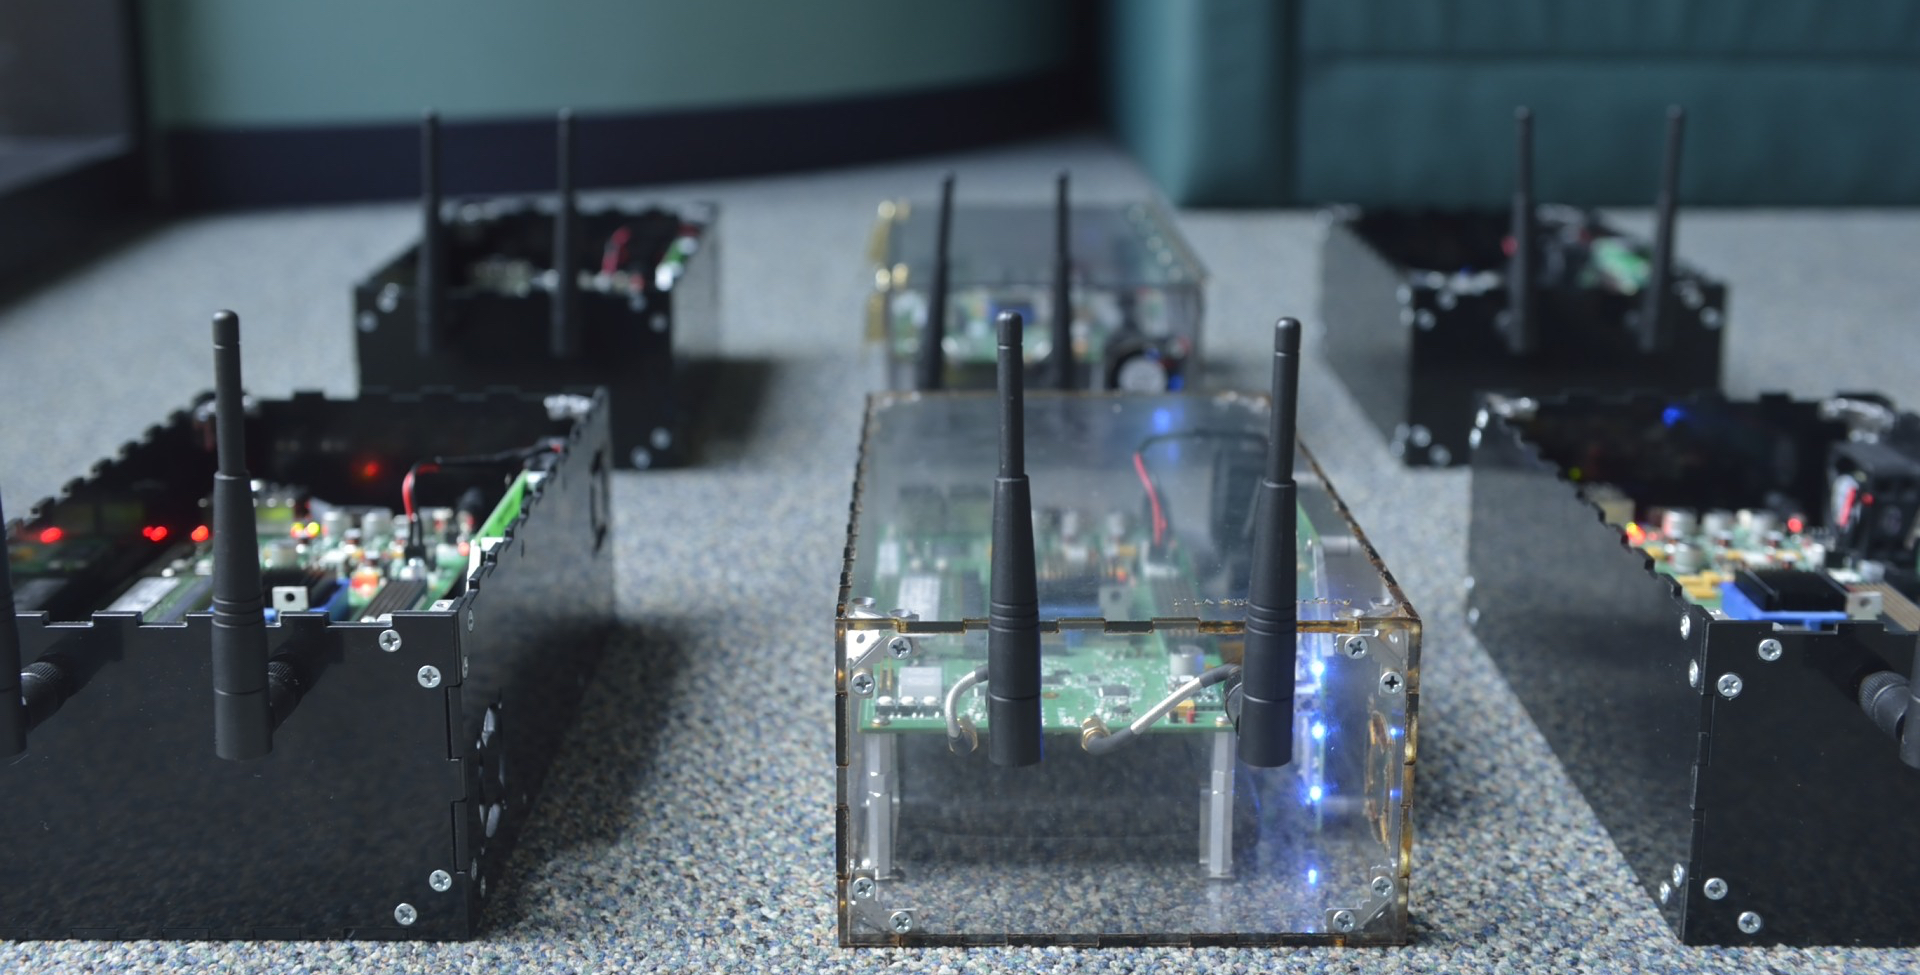
\includegraphics[width=0.95\textwidth]{ArgosMobile}
  \vspace{-2mm}
\caption{\emph{Battery-powered ArgosMobile based WARPv3.}}
\label{fig:argosmobile}
\end{minipage}
\hspace{+3mm}
\begin{minipage}[t][6cm]{0.463\textwidth}
    \centering
 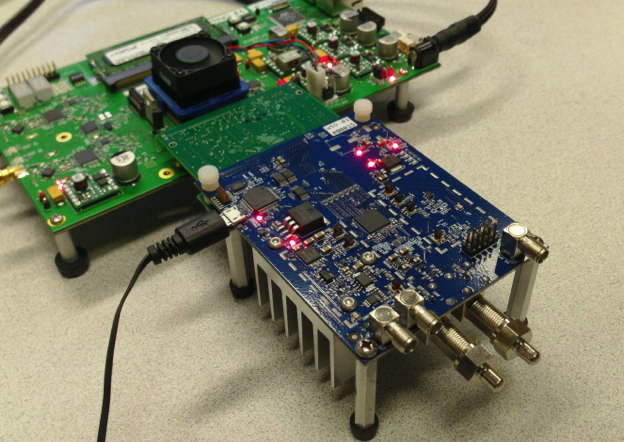
\includegraphics[width=0.95\textwidth]{WSD}
		\vspace{-2mm}
    \caption{\it{Volo wireless Whitespace daughtercard (WSD) adds UHF support to ArgosNet.}}
    \label{fig:WSD}
\end{minipage}
\vspace{-1mm}
\end{figure*}